\subsection{Моделирование на основе кинетической теории транспорта}
Моделирование на основе кинетической теории транспорта заключается в решении кинетического уравнения Больцмана, описывающего распространение электронов в структуре. Этот метод успешно применяется для моделирования рассеяния электронного пучка в планарных структурах, состоящих из небольшого количества слоев~\cite{Stepanova_2006, Stepanova_2010}. Для задач с более сложной геометрией необходимо введение дополнительных граничных условий, что значительно усложняет расчет.


\paragraph{Определение распределения электронов по глубине} \mbox{} \\
\indent В большинстве случаев для упрощения расчетов, рассматривается точечный (в плоскости $XY$) пучок электронов, направленный под прямым углом к поверхности (вдоль оси $Z$). Распространение электронов в веществе по глубине может быть описано функцией распределения $f(z, E, \cos \theta_v)$, где $z$, $E$ -- глубина проникновения электрона в образец и его энергия, $\cos \theta_v$ -- угол между скоростью электрона и осью $z$. В этом случае уравнение Больцмана принимает вид~\cite{ME_rev_60}:
\begin{equation} \label{eq:Boltzman_1}
	\frac{d E}{d s} \frac{\partial f}{\partial E}+\cos \theta_v \frac{\partial f}{\partial z}=\frac{1}{\Lambda} \int w(\cos \gamma)\left[f\left(\cos \theta_{v^{\prime}}\right)-f\left(\cos \theta_v\right)\right] d \Omega_\gamma,
\end{equation}
где $\frac{dE}{ds}$ -- потери энергии на единицу длины пути, $\Lambda$ -- длина свободного пробега при упругом рассеянии, $v$ и $v^{\prime}$ -- скорости до и после рассеяния, соответственно, $w(\cos \gamma)$ -- нормированное дифференциальное сечение упругого рассеяния на угол $\gamma$:
\begin{equation} \label{eq:Boltzman_2}
	w(\cos \gamma)=\frac{1}{\sigma_{\mathrm{el}}} \frac{d \sigma}{d \Omega_\gamma}.
\end{equation}
Уравнение \ref{eq:Boltzman_1} может быть решено в диффузионном приближении~\cite{ME_rev_61}, применимом в диапазоне энергий, характерных для электронно-лучевой литографии. Для этого функция распределения электронов раскладывается в ряд по полиномам Лежандра $P(\cos \theta)$:
\begin{equation} \label{eq:Boltzman_3}
	f\left(z, E, \cos \theta_v\right)=\sum_0^{\infty} C_n(z, E) P_n\left(\cos \theta_n\right).
\end{equation}
Подстановка \ref{eq:Boltzman_3} в \ref{eq:Boltzman_1} приводит к дифференциальной разностной схеме для коэффициентов $C_n$:
\begin{equation} \label{eq:Boltzman_4}
	\left(\frac{d E}{d s}\right) \frac{\partial C_n}{\partial E}+\frac{n}{2 n-1} \frac{\partial C_{n-1}}{\partial z}+\frac{n+1}{2 n+3} \frac{\partial C_{n+1}}{\partial z}=-\frac{1}{\lambda_n} C_n,
\end{equation}
где
\begin{equation} \label{eq:Boltzman_5}
	\frac{1}{\lambda_n}=\frac{1}{\Lambda} \int\left[1-P_n(\cos \gamma)\right] W(\cos \gamma) d \Omega_\gamma.
\end{equation}
Коэффициенты $C_0$ и $C_1$ пропорциональны плотности вероятности и проекции плотности потока вероятности на ось $z$, соответственно:
\begin{equation} \label{eq:Boltzman_6}
	\begin{gathered}
		\rho(z, E)=\int f\left(z, E, \cos \theta_v\right) d \Omega_v=4 \pi C_0(z, E), \\
		J_z(z, E)=\int v \cos \theta_v f\left(z, E, \cos \theta_v\right) d \Omega_v=\frac{4 \pi}{3} v C_1(z, E).
	\end{gathered}
\end{equation}
Точное решение \ref{eq:Boltzman_1} возможно при отбрасывании в  коэффициентов $C_n$ с \break $n>1$, соответствующих турбулентному движению. При этом уравнение~\ref{eq:Boltzman_4} принимает вид уравнения диффузии:
\begin{equation} \label{eq:Boltzman_7}
	\frac{\partial}{\partial E} \rho(z, E)=a(E) \frac{\partial^2}{\partial z^2} \rho(z, E), a(E)=\left(\frac{d E}{d s}\right)^{-1} \frac{\lambda_1}{3}.
\end{equation}
Его решение:
\begin{equation} \label{eq:Boltzman_8}
	\rho(z, E)=\frac{1}{\sqrt{\pi} \sigma(E)} \exp \left(-\frac{z^2}{4 \sigma^2(E)}\right)\left\{1-\frac{\sqrt{\pi} \sigma(E)}{\Delta \lambda_1\left(E_0\right)} \exp \left(\zeta^2\right) \operatorname{erfc}\left(\zeta^2\right)\right\},
\end{equation}
где
\begin{equation} \label{eq:Boltzman_9}
	\zeta = \frac{z}{2 \sigma(E)}+\frac{\sigma(E)}{\Delta \lambda_1\left(E_0\right)}, \quad \sigma^2=\int a(E) d E, \quad \Delta=0.71.
\end{equation}
Для описания функции распределения электронов в системе, состоящей из нескольких слоев, решение для предыдущего слоя используется как граничное условие для уравнения диффузии в новом слое.


\paragraph{Определение латерального распределения электронов} \mbox{} \\
\indent Латеральное распределение электронов описывается функцией плотности вероятности $\rho(r, z, E)$, определяющей вероятность нахождения электрона с энергией $E$ в кольце радиуса $r$, имеющем объем $2 \pi r dr dz$ и расположенном параллельно поверхности резиста на глубине $z$. Для определения продольного распределения электронов необходимо решение уравнения Больцмана в более общем виде, чем \ref{eq:Boltzman_1}~\cite{ME_rev_63}, и при этом отдельно учитывается вклад от электронов, рассеянных на малые углы (индекс ``$\mathrm{f}$''), обратно рассеянных электронов (индексы ``$\mathrm{bd}$'' и ``$\mathrm{bs}$'') и вторичных электронов (индекс ``$\mathrm{s}$'')~\cite{ME_rev_64}:
\begin{equation} \label{eq:Boltzman_10}
	\rho(r, z, E)=\rho(z, E)\left[\rho_\mathrm{f}(r \mid z, E)+\rho_\mathrm{bd}(r \mid z, E)\right]+\rho_\mathrm{bs}(r, z, E)+\rho_\mathrm{s}(r, z, E).
\end{equation}
Здесь выражения вида $\rho(r|z,E)$ означают плотность вероятности при известных значениях $z$ и $E$. Слагаемое $\rho_\mathrm{f}(r|z,E)$ описывает продольное уширение пучка за счет небольшого количества актов рассеяния первичных электронов на малые углы в слое резиста:
\begin{equation} \label{eq:Boltzman_11}
	\rho_f(r \mid z, E)=\frac{3 \lambda_1}{2 \pi z^3} \exp \left(-\frac{3 \lambda_1 r^2}{2 z^3}\right),
\end{equation}
где $\lambda_1$ определяется из соотношения \ref{eq:Boltzman_5}.

Обратное рассеяние электронов происходит за счет рассеяния на большие углы вблизи границы резиста с подложкой ($\rho_\mathrm{bs}$), либо за счет диффузии электронов в структуре ($\rho_\mathrm{bd}$):
\begin{equation} \label{eq:Boltzman_12}
	\begin{gathered}
		\rho_\mathrm{bs}(r, z, E)=\frac{1}{\pi} \int_z^{z_\mathrm{d}} \beta(1+\beta) \rho\left(z^{\prime}, E\right) \frac{z^{\prime}-z}{R} \frac{d z^{\prime} / \Lambda}{\left[(1+\beta) R+z^{\prime}-z\right]^2}, \\
		\rho_\mathrm{bd}(r \mid z, E)=\frac{A^2}{3} \int_{z_\mathrm{d}}^{z_\mathrm{max}}\left(\frac{1}{4 \pi \sigma_\mathrm{b}^2}\right)^{3 / 2} \exp \left(-\frac{R^2}{4 \sigma_\mathrm{b}^2}\right) \frac{z^{\prime}-z}{z_{\max }-z_\mathrm{d}} d z^{\prime},\\
		R=\sqrt{r^2+\left(z-z^{\prime}\right)^2}, \\ \sigma_\mathrm{b}^2=\int_{E\left(z^{\prime}\right)}^{E(z)} a\left(E^{\prime}\right) d E^{\prime},
	\end{gathered}
\end{equation}
где $\beta$ -- параметр экранирования в формуле Резерфорда для дифференциального сечения упругого рассеяния, $\Lambda$ -- длина свободного пробега при упругом рассеянии, $a(E)$ -- коэффициент диффузии в уравнении~\ref{eq:Boltzman_7}, $E(z)$ , $E(z^\prime)$ -- средние энергии электрона, получаемые за счет интегрировании функции $Ef(z, E, \cos \theta_v )$. Параметр $z_\mathrm{d}$ выражает максимальную глубину проникновения электронов, рассеивающихся на большие углы вблизи границы резиста с подложкой, и его значение подбирается на основе моделирования методом Монте-Карло. Значения параметров $z_\mathrm{max}$ и $A$, определяющих максимальную глубину, на которой могут находиться обратно отраженные электроны, и коэффициент обратного отражения электронов соответственно, также выбираются исходя из результатов моделирования методом Монте-Карло. Например, для слоя полиметилметакрилата (ПММА) толщиной 0.5 мкм на кремниевой подложке используются следующие значения этих параметров: $z_\mathrm{d}$ = 0.83 мкм, $z_\mathrm{max}$ = 8.5 мкм, $A$ = 0.19.

Уширение пучка за счет генерации вторичных электронов описывается функцией плотности вероятности для вторичных электронов:
\begin{equation} \label{eq:Boltzman_13_0}
	\begin{split}
		\rho_\mathrm{s}(r, z, E) = \int_{2 E}^{E_0} d E^{\prime} & p_\mathrm{inel} \left(E^{\prime}\right) \Phi\left(E, E^{\prime}\right) \times \\
		& \times \int d^3 \vec{r}^{\prime} \frac{1}{8 \pi S^3(E)} \exp \left(\frac{-\left|\vec{r}-\vec{r}^{\prime}\right|}{S(E)}\right) \rho\left(r^{\prime}, z, E^{\prime}\right).
	\end{split}
\end{equation}
Здесь $E_0$ -- начальная энергия электронов, $p_\mathrm{inel}$ -- вероятность неупругого рассеяния с генерацией вторичного электрона, определяемая на основе сечений упругого и неупругого рассеяния ($\sigma_\mathrm{el}(E)$ и $\sigma_\mathrm{inel}(E)$, соответственно):
\begin{equation} \label{eq:Boltzman_13}
	p_\mathrm{inel}(E) = \frac{\sigma_\mathrm{inel}}{\sigma_\mathrm{el}+\sigma_\mathrm{inel}}.
\end{equation}
Функция $\Phi\left(E, E^{\prime}\right)$ представляет собою дифференциальное сечение неупругого рассеяния, нормированное на полное сечение неупругого рассеяния, $S(E)$ -- максимальная глубина проникновения электронов, выражаемая через потери энергии на единицу пути:
\begin{equation} \label{eq:Boltzman_14}
	S(E)=\int_{E_0}^{E_{\min }} d E\left(\frac{d E}{d s}\right)^{-1}.
\end{equation}

Одним из наиболее важных результатов моделирования в этом случае является распределение энергии, выделившейся в резисте при экспонировании. Плотность выделившейся энергии в пересчете на один первичный электрон может быть получена за счет интегрирования произведения плотности вероятности и функции потерь энергии~\cite{ME_rev_64}.


\subsection{Моделирование методом Монте-Карло}
В отличие от моделирования на основе кинетической теории транспорта, при моделировании методом Монте-Карло траектория каждого первичного или вторичного электрона рассчитывается отдельно. Параметры траектории и потери энергии электрона определяются на основе дифференциальных сечений процессов упругого и неупругого рассеяния с использованием случайных чисел, равномерно распределенных на промежутке [0, 1). Данный метод требует больших вычислительных мощностей, чем вышеописанный метод моделирования на основе кинетической теории транспорта, но при этом его сложность практически не зависит от формы структуры и количества входящих в нее материалов. Также, в отличие от моделирования на основе кинетической теории транспорта, моделирование рассеяния электронного пучка в веществе методом Монте-Карло позволяет воспроизвести стохастический характер процессов рассеяния.

\paragraph{Определение длины пробега электрона} \mbox{} \\
\indent Полные сечения процессов упругого и неупругого рассеяния электронов в веществе вычисляются путем интегрирования дифференциальных сечений соответствующих процессов:
\begin{equation} \label{eq:MC_1}
	\sigma_\mathrm{el/inel}(E) = \int_Q \frac{d \sigma_\mathrm{el/inel}(E, q)}{dq} dq,
\end{equation}
где индекс ``$\mathrm{el/inel}$'' обозначает тип рассеяния -- упругое рассеяние или неупругое, соответственно. Дифференциальные сечения рассеяния зависят как от энергии налетающего электрона, так и от второй переменной, которая здесь называется $q$. Для упругого рассеяния это полярный угол рассеяния $\theta$, для неупругого -- энергия $\Delta E$, передаваемая налетающим электроном среде. Интегрирование в формуле \ref{eq:MC_1} производится по области всех возможных значений $q$. Далее длина свободного пробега электрона в веществе определяется по формуле
\begin{equation} \label{eq:MC_4}
	\lambda^{-1}(E) = \lambda_\mathrm{el}^{-1}(E)+\lambda_\mathrm{inel}^{-1}(E),
\end{equation}
где
\begin{equation} \label{eq:MC_3}
	\lambda_\mathrm{el/inel}(E)=\left(n \sigma_\mathrm{el/inel}(E)\right)^{-1},
\end{equation}
$n$ -- концентрация рассеивающих центров в веществе.

Вероятность того, что на промежутке пути длиной $s$ не произойдет рассеяния, равна~\cite{ME_rev_49}
\begin{equation} \label{eq:MC_5}
	p(s) = \lambda(E)^{-1} \exp \left(-\frac{s}{\lambda(E)}\right).
\end{equation}
Длина пробега электрона может быть определена по формуле
\begin{equation} \label{eq:MC_6}
	s = -\lambda(E) \ln \left(\xi_1\right),
\end{equation}
где $\xi_1$ случайное число из промежутка [0, 1). Если пробег электрона начинается и заканчивается в слоях, состоящих из разного вещества (например, моделирование производится для системы из $m$ слоев с толщинами $s_1$, $s_2$, ..., $s_m$ и длинами свободного пробега электронов $\lambda_1$, $\lambda_2$, ..., $\lambda_m$), длина пробега электрона s должна быть пересчитана с условием пересечения границы между слоями. Например, она может быть вычислена как верхний предел интегрирования в формуле~\cite{Han_2002}
\begin{equation} \label{eq:MC_7}
	\ln \left(\xi_1\right)=-\frac{s_1}{\lambda_1}-\frac{s_2}{\lambda_2} \ldots+\int_{s_k}^s-\frac{d u}{\lambda_k},
\end{equation}
где $k \leq m$.


\paragraph{Определение типа взаимодействия} \mbox{} \\
\indent Далее на основе вероятностей упругого и неупругого рассеяния
\begin{equation} \label{eq:MC_8}
	p_\mathrm{el/inel}=\sigma_\mathrm{el/inel} /\left(\sigma_\mathrm{el}+\sigma_\mathrm{inel} \right)
\end{equation}
определяется тип взаимодействия (упругое или неупругое рассеяние), в котором электрон примет участие после прохождения пути $s$:
\begin{equation} \label{eq:MC_9}
	\begin{split}
		\xi_2 < p_\mathrm{el} & \Rightarrow \text{упругое рассеяние} \\
		\xi_2 \geq p_\mathrm{el} & \Rightarrow \text{неупругое рассеяние}
	\end{split}
\end{equation}
где $\xi_2$ -- новое случайное число из промежутка [0, 1).


\paragraph{Определение нового направления электрона и потерь энергии} \mbox{} \\
\indent В случае упругого рассеяния определяется новое направление рассеянного электрона, для чего используются случайные числа $\xi_3$ и $\xi_4$. Азимутальный угол рассеяния $\varphi$ считается равномерно распределенным на промежутке [0,~2$\pi$) и определяется выражением
\begin{equation} \label{eq:MC_11}
	\varphi = 2 \pi \xi_3.
\end{equation}
Полярный угол рассеяния $\theta$ вычисляется на основе дифференциального сечения упругого рассеяния по формуле
\begin{equation} \label{eq:MC_12}
	\xi_4 = \frac
	{\displaystyle \int_0^\theta \frac{d \sigma}{d \Omega} \sin \vartheta d \vartheta}
	{\displaystyle \int_0^\pi \frac{d \sigma}{d \Omega} \sin \vartheta d \vartheta}.
\end{equation}
При известных углах $n$-ого акта рассеяния $\varphi_n$ и $\theta_n$ новое направление движения электрона $\vec{x}_n$ задается ортом вдоль начального направлением движения электрона $\vec{x_0}$ и комбинацией матриц поворота~\cite{rotation_matrices}:
\begin{equation} \label{eq:MC_13}
	\vec{x}_n=O_n^T \vec{x}_0, \quad O_n=W_n O_{n-1},
\end{equation}
\begin{equation} \label{eq:MC_14}
	W_n=\left(\begin{array}{ccc}
		\cos \varphi_n & \sin \varphi_n & 0 \\
		-\sin \varphi_n \cos \theta_n & \cos \varphi_n \sin \theta_n & \sin \theta_n \\
		\sin \varphi_n \sin \theta_n & -\cos \varphi_n \sin \theta_n & \cos \theta_n
	\end{array}\right).
\end{equation}
При этом используются начальные значения $O_{-1}$ = $E$ (единичная матрица) и $\varphi_0$ = $\theta_0$ = 0.

В случае неупругого рассеяния определяются потери энергии. При использовании модели непрерывных потерь энергии потери энергии на пути $s$, определяемом выражением \ref{eq:MC_6} , вычисляются по формуле
\begin{equation} \label{eq:MC_15}
	\Delta E=\int_0^s \frac{d E}{d s} d s \approx \frac{d E}{d s} s.
\end{equation}
При использовании модели дискретных потерь энергии потери энергии $\Delta E$ определяются на основе случайного числа $\xi_5$:
\begin{equation} \label{eq:MC_16}
	\xi_5 = \frac
	{\displaystyle \int_{E_\mathrm{min}}^{\Delta E} \frac{d \sigma}{d\left(\Delta E^{\prime}\right)} d\left(\Delta E^{\prime}\right)}
	{\displaystyle \int_{E_\mathrm{min}}^{E_\mathrm{max}} \frac{d \sigma}{d\left(\Delta E^{\prime}\right)} d\left(\Delta E^{\prime}\right)},
\end{equation}
где дифференциальные сечения неупругого рассеяния $\displaystyle{\frac{d \sigma}{d \Delta E}}$ вычисляются по формуле Гризинского или из диэлектрической функции, а значения $E_\mathrm{min}$ и $E_\mathrm{max}$ принимаются равными $0$ и $E/2$ соответственно~\cite{Dapor_large_book}. Пример траектории электрона в веществе, промоделированной методом Монте-Карло, приведен на рисунке~\ref{fig:Monte_Carlo_scheme}.

\begin{figure}[h]
	\centering
	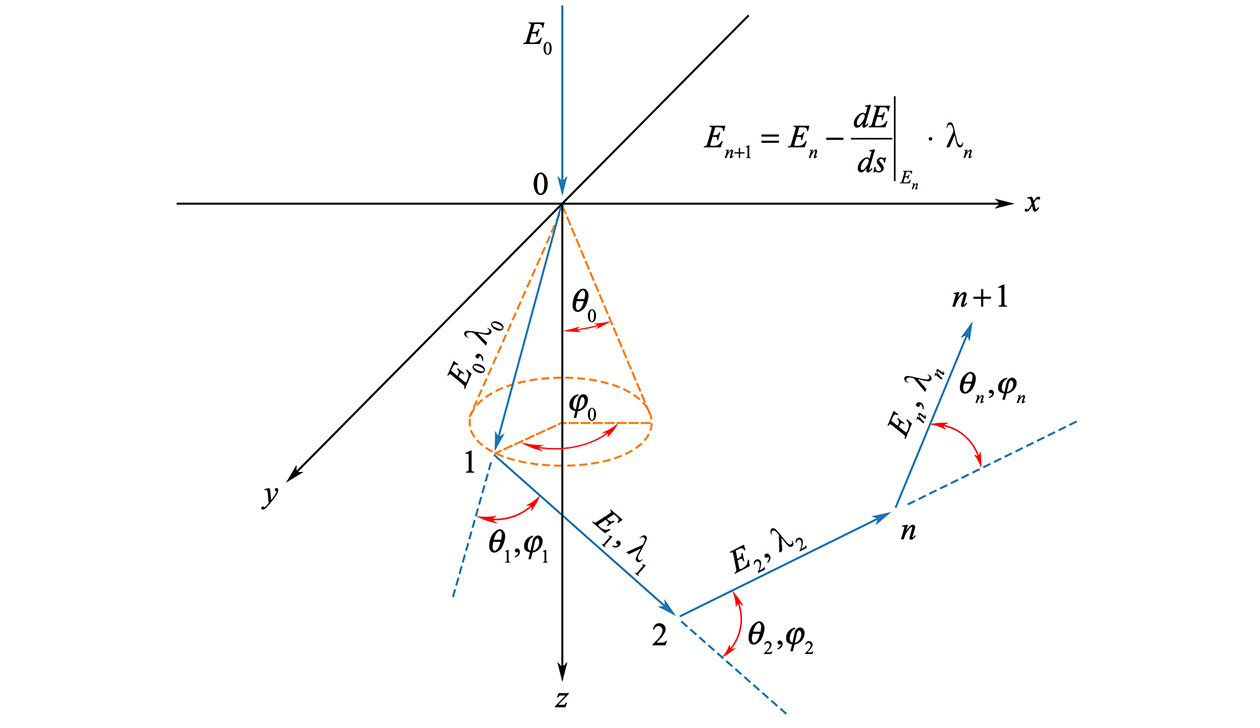
\includegraphics[width=\linewidth]{jpg/MC_200}
	\vspace{-0.5em}
	\caption{Схематическое изображение траектории электрона в веществе, получаемой при моделировании методом Монте-Карло в случае использования модели непрерывных потерь энергии.\vspace{1.5em}}
	\label{fig:Monte_Carlo_scheme}
\end{figure}
